% Based on template by MR

\documentclass[12pt,twoside,notitlepage]{report}

\usepackage{a4}
\usepackage{verbatim}
\usepackage{natbib}
\usepackage{graphicx}
\usepackage{algorithm}

\input{epsf}                            % to allow postscript inclusions

\raggedbottom                           % try to avoid widows and orphans
\sloppy
\clubpenalty1000%
\widowpenalty1000%

\addtolength{\oddsidemargin}{6mm}       % adjust margins
\addtolength{\evensidemargin}{-8mm}

\renewcommand{\baselinestretch}{1.1}    % adjust line spacing to make
                                        % more readable

% Resize over-large graphics ( http://tex.stackexchange.com/questions/27083/can-i-conditionally-scale-an-image-with-graphicx )
\newcommand{\lwincludegraphics}[2][]{%
  \sbox{0}{\includegraphics[#1]{#2}}%
  \ifdim\wd0>\linewidth
    \resizebox{\linewidth}{!}{\box0 }%
  \else
    \leavevmode\box0
  \fi}

\newcommand{\msg}[1] {{\bf #1}}         % \msg command for formatting Paxos messages
\newcommand{\op}[1]  {{\bf #1}}         % \op  command for formatting database operations


\begin{document}

\bibliographystyle{plain}


%%%%%%%%%%%%%%%%%%%%%%%%%%%%%%%%%%%%%%%%%%%%%%%%%%%%%%%%%%%%%%%%%%%%%%%%
% Title


\pagestyle{empty}

\hfill{\LARGE \bf Charlie Shepherd}

\vspace*{60mm}
\begin{center}
\Huge
{\bf PDB: A Distributed Database Based on Paxos} \\
\vspace*{5mm}
Computer Science Tripos \\
\vspace*{5mm}
Churchill College \\
\vspace*{5mm}
\today  % today's date
\end{center}

\cleardoublepage

%%%%%%%%%%%%%%%%%%%%%%%%%%%%%%%%%%%%%%%%%%%%%%%%%%%%%%%%%%%%%%%%%%%%%%%%%%%%%%
% Proforma, table of contents and list of figures

\setcounter{page}{1}
\pagenumbering{roman}
\pagestyle{plain}

\chapter*{Proforma}

{\large
\begin{tabular}{ll}
Name:               & \bf Charlie Shepherd                        \\
College:            & \bf Churchill College                     \\
Project Title:      & \bf PDB: A Distributed Database Based on Paxos \\
Examination:        & \bf Computer Science Tripos, July 2013        \\
Word Count:         & \bf wordcount \\
Project Originator: & Charlie Shepherd                    \\
Supervisor:         & Stephen Cross                    \\
\end{tabular}
}


\section*{Original Aims of the Project}

\subsection*{Project aims}

I aim to implement a distributed database. This will be based on the Paxos protocol.

\subsubsection*{Paxos}

The first half of the project is to implement the Paxos protocol. This will be done in a module,
providing an interface which the database can then use to 

The project must correctly implement the Paxos protocol.  The library must be capable of forming a
running network, in particular dynamic leader election, as well as achieving consensus on a
key/value store across the network.

The database must implement a subset of SQL, specifically. The database must have all ACID
properties, that is.

\section*{Work Completed}

All that has been completed appears in this dissertation.

\section*{Special Difficulties}

None.

\newpage
\section*{Declaration}

I, Charlie Shepherd of Churchill College, being a candidate for Part II of the Computer Science
Tripos, hereby declare that this dissertation and the work described in it are my own work,
unaided except as may be specified below, and that the dissertation does not contain material that
has already been used to any substantial extent for a comparable purpose.

\bigskip
\leftline{Signed: }

\medskip
\leftline{Date: \today}

\cleardoublepage

\tableofcontents

\listoffigures

\newpage
\section*{Acknowledgements}

Acknowledge various people

%%%%%%%%%%%%%%%%%%%%%%%%%%%%%%%%%%%%%%%%%%%%%%%%%%%%%%%%%%%%%%%%%%%%%%%
% now for the chapters

\cleardoublepage        % just to make sure before the page numbering
                        % is changed

\setcounter{page}{1}
\pagenumbering{arabic}
\pagestyle{headings}

\chapter{Introduction}

\section{Overview}

I set out to build a distributed database with ACID properties, based on the Paxos protocol. Paxos
was first described in Leslie Lamport's paper \emph{The Part Time Parliament} \cite{lamport98}.

\section{Motivation}

% XXX: finish!

\section{Distributed Consensus Problem}

Consensus is an integral problem in distributed systems. The consensus problem is that of getting
all nodes in a distributed system to agree on a value. Formally, an algorithm that satisfies the
consensus problem satisfies three properties:

\begin{enumerate}
\item Agreement - all nodes must decide the same value.
\item Validity - the value that is decided upon must have been proposed by some node in the
	network.
\item Termination - all nodes eventually decide on a value.
\end{enumerate}

Decision is defined as follows - a process must decide on a value only once, and cannot change the
value once it has been decided.

\subsection*{Failure Modes}

Distributed networks must be able to deal with failure in a number of forms. Nodes may fail and
stop executing completely, this is known as the \emph{fail-stop} model. In practice, a more accurate
model is the \emph{fail-recover} model. This is where a node stops executing, then resumes execution
at a later time. This more accurately models real life, where asynchronous networks mean that it
may take an arbitrarily long time to receive a message, and that messages may arrive out of order
or not at all. The most general failure model is that of \emph{Byzantine failure}, where nodes may
respond incorrectly or even deliberately lie in order to mislead the protocol. In practice this is
unlikely, and can be mediated using checksums, message digests and authentication. In the
Preparation chapter I will go into detail about the types of failure that my database can handle.

\subsection*{2 Phase Commit}

\begin{figure}[h!]
\centering
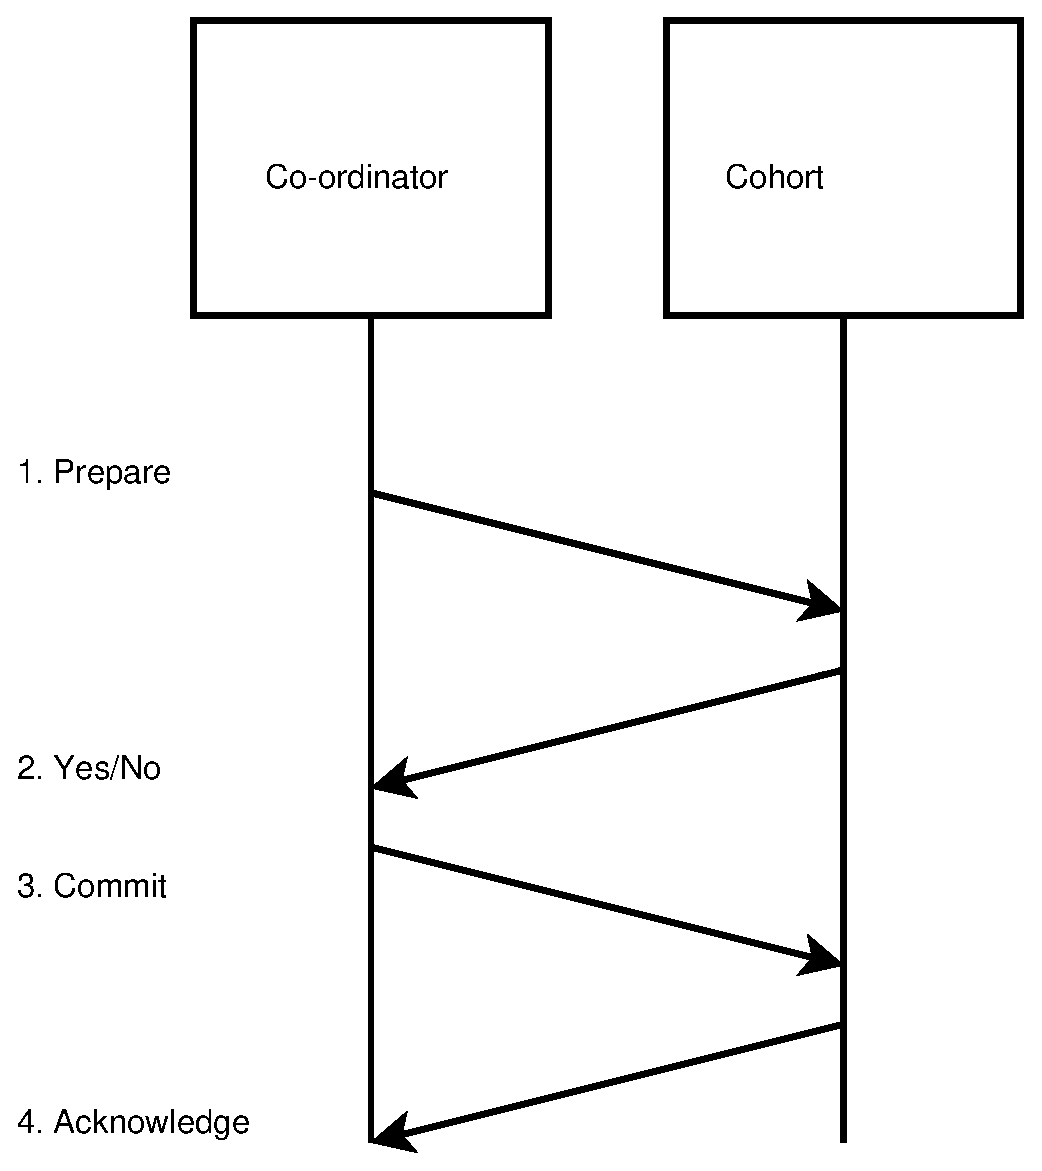
\includegraphics[scale=0.5]{figs/two-pc.eps}
\caption{\label{fig:two-pc}Two Phase Commit}
\end{figure}

2 Phase Commit (2PC) is one of the simplest consensus protocol, and one of the most brittle. The
basic message flow is shown in figure~\ref{fig:two-pc}. It has two phases:

\begin{enumerate}
\item The co-ordinator (the node initiating the protocol) sends a \msg{PROPOSE} message to each
	node in a cohort of size $N$, asking them to accept the value proposed.
\item The nodes reply with a \msg{YES} or \msg{NO} reply.
\item If all nodes respond with a \msg{YES} message, the co-ordinator sends a \msg{CONFIRM} message. Otherwise, if
	any node responds with a \msg{NO} message, it sends an \msg{ABORT} message to all nodes.
\item Nodes reply with an \msg{ACK} message, and the co-ordinator marks the transaction as
	complete when all nodes have acknowledged it.
\end{enumerate}

2PC solves the consensus problem in a failure free network. However if we can have failures then
the protocol can suffer from a number of limitations. If the co-ordinator crashes before sending
any messages, we satisfy consensus trivially. However, if the co-ordinator crashes after sending
$x$ messages, where $1 \le x < N$, the protocol cannot continue - it is blocked on the
co-ordinator resuming, and if it never resumes then some members of the cohort are blocked
permanently. In fact, once a node has sent a \msg{YES} message, it is blocked until it receives a
response. This is a big disadvantage for a concurrent system. While there are extensions to
resolve the problem of a crashing co-ordinator, these do not fix the fundamental problem of using
a blocking protocol in an asynchronous network. (These extensions often involve a ``watchdog'' or
``recovery node'' This is still not a satisfactory solution as the simultaneous crash of the
co-ordinator and a cohort member means the state of the network is not recoverable (ie, we cannot
tell if the cohort member who crashed voted \msg{YES} or \msg{NO}.))

\subsection*{3 Phase Commit}

\begin{figure}[h!]
\centering
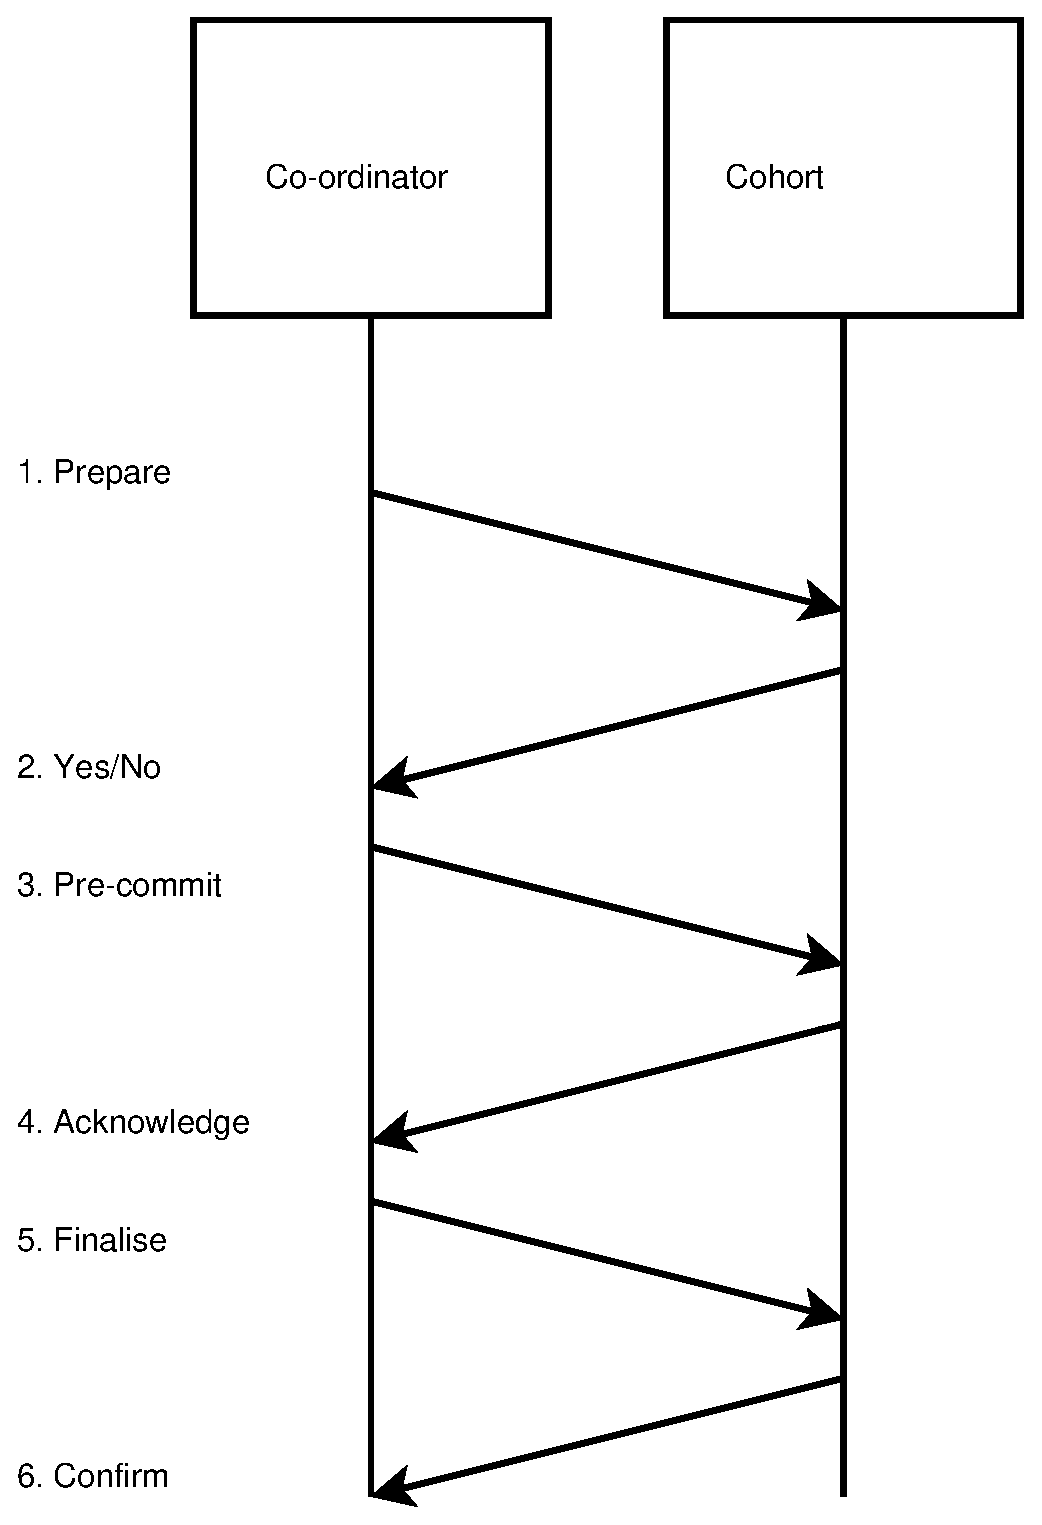
\includegraphics[scale=0.5]{figs/three-pc.eps}
\caption{\label{fig:three-pc}Three Phase Commit}
\end{figure}

3 Phase Commit (3PC) is a modification of 2PC that turns it from a synchronous protocol into an
asynchronous protocol. This is done by adding a third phase, so that we can use timeouts to assert
the state of the system at any point in time. Again the basic message flow is shown in
figure~\ref{fig:three-pc}. The three phases are:

\begin{enumerate}
\item \msg{Prepare}: the co-ordinator asks the cohort members if they can perform the operation. At
	this stage if there is a failure or timeout, the co-ordinator aborts the transaction.
\item The cohort respond with a \msg{YES} or \msg{NO}. Again, if there is a failure or timeout the cohort
	member considers the transaction aborted.
\item \msg{Pre-commit}: If the co-ordinator receives \msg{YES} messages from every member of the
	cohort, it sends a \msg{Pre-commit} message to them all, otherwise it aborts the
	transaction. It also aborts in the case of a failure or timeout.
\item \msg{Acknowledge}: If the cohort member recieves a \msg{Pre-commit} message, it replies with
	an \msg{Acknowledge} message. If the co-ordinator aborts, or there is a failure or
	timeout, the cohort member aborts.
\item \msg{Finalise}: If the co-ordinator times out, it aborts the transaction. Otherwise, when it
	has received \msg{Acknowledge} messages from every cohort member it sends a \msg{Finalise}
	message to them all.
\item \msg{Confirm}: Once a cohort member has received a \msg{Finalise} message, it commits the
	transaction, even if the co-ordinator fails. It can reply with a \msg{Confirm} message.
\end{enumerate}

This fixes the problem of node failure, but still suffers from a significant problem. If there is
a network partition, and all nodes who voted \msg{YES} are in one half and all nodes who voted
\msg{NO} are in the other, both partitions will recover into different, inconsistent states.
Brewer's CAP theorem \cite{gilbert2002} says that we cannot achieve both consensus and availability
during a network partition - we must choose one. 3PC opts for availability, but for a distributed
database with ACID properties it is preferable to have consensus. Paxos guarantees consensus at
the cost of lack of availability in a network partition.

\subsection*{Paxos}

Paxos is a generalisation of 2PC and 3PC that handles more failure modes. While 3PC can handle
failures, it only handles \emph{fail-stop} failures, not \emph{fail-recover} failures. This is
unfortunate, as computer networks are asynchronous networks, and can therefore be modelled using a
fail-recover model to account for arbitrary delays from messages being sent to being received
(fail-stop would mean messages can only be dropped, not delayed for an arbitrary length of time).

Another key advantage of Paxos is that it can guarantee consistency during network partitions,
unlike 3PC which gives availability instead. However, one potential drawback of Paxos is that it
sacrifices \emph{liveness}, that is, the guarantee that it will make progress. This means that
there is no upper bound on the time it will take Paxos to achieve consensus (ie, it may never
terminate). This is due to the FLP impossibility proof \cite{fischer85}, and in practise is not a serious concern.

\section{Databases}

\subsection*{ACID}

Commonly all databases provide ACID properties. ACID stands for:

\begin{itemize}
\item Atomic - an operation is either performed or is not performed.
\item Consistent - the database remains in a consistent state at all times.
\item Isolated - one operation cannot see the intermediate state due to another operation occurring
	at the same time.
\item Durable - once an operation is ``committed'' it is permanently stored - the effects of it will
	not be lost.
\end{itemize}

There are many reasons why ACID is a key requirement of most databases. ACID makes it far easier
for application developers to reason about concurrency in a system where there may be multiple
clients reading and writing the same data simultaneously. It also enable effective abstraction, as
the atomicity requirement in particular gives the well defined characteristics when an operation
or transaction fails. ACID also provides clear guarantees with regard to data stability and
longevity, in particular how this relates to consistency, so that users can be clear as to the
overall state of the system.

\subsection*{Centralisation vs Distributed}

Databases are generally found in one of two topologies - centralised or distributed. These
different topologies are used in different situations and to different ends.

A centralised database is a single node in a single location.
In general, centralised databases are simpler in design and on the whole faster than distributed
databases.
Many general properties of centralised vs. distributed systems apply to centralised databases -
they are easier to perform organise, to edit, to query and to backup. May slow down under load. It
is easier to maintain the integrity of data on a centralised database, as there is only one
``current'' version of the data under consideration.

In contrast, distributed databases are more resilient and scalable than centralised databases.
There is no longer a single point of failure, and they can be extended by adding nodes, although
this will have a point of diminishing returns. Distributed databases are often more complex in
design, as they have to ensure consistency between nodes (although there is a recent trend to
relax this constraint in certain ``NoSQL'' databases. Here I will only consider traditional RDBMS
systems). In particular, distributed databases can be slow accessing non local data.

\subsection*{Existing Paxos databases}

Paxos has recently become a very popular algorithm for ensuring distributed
consensus. One good example is Google using Paxos for a distributed lock
service called ``Chubby'' \cite{chandra07}. This underpins their BigTable
distributed database which is used across Google.

Apache Zookeeper, a centralised service for providing distributed services such
as synchronisation, naming and configuration management, also uses a Paxos
based protocol called ZAB.

\cleardoublepage

\chapter{Preparation}

\section{Paxos}

\subsection{Introduction}

Paxos is a distributed consensus protocol. It was developed by Leslie Lamport at Microsoft
research when he was trying to disprove its existence. Paxos is failure tolerant for up to $F$
simultaneous failures in a network of $2F + 1$ nodes.

Paxos is actually a family of protocols, based around the same main algorithm. The Paxos algorithm
is an algorithm for agreeing on a single value across a network of processors. Paxos provides
three guarantees: safety, liveness and non-triviality:

\begin{enumerate}
	\item Consistency: Only one value is chosen.
% XXX: wtf, how can we guarantee liveness, yet liveness is impossible??
	\item Liveness: If a value is proposed, eventually some value is chosen.
	\item Non-triviality: only proposed values may be chosen.
\end{enumerate}

Paxos can tolerate certain kinds of failures. These are: messages being delivered late or not at
all, etc XXX.

However Paxos cannot tolerate ``rogue'' processes, that is, processes deliberately sending malicious
or incorrect messages. There is a variant of Paxos called \emph{Byzantine Paxos} which can tolerate this,
albeit at a failure tolerance of $F$ for $3F + 1$ nodes. I will not go into this variant further
in this dissertation.

\subsection{Definitions}

\subsubsection*{Proposal Numbering}

One of the assumptions that Paxos makes is that every proposal has a unique proposal number. This
is necessary so that proposals have a \emph{total order}, ie we can compare any two proposals to
find the maximum ordered proposal. The conventional way to achieve this is to define a proposal
number as a 2-tuple of (sequence number, node address). These can be compared lexicographically,
and as node addresses are unique, every proposal number will be unique. In practice I plan to use
UUIDs as node identifiers, in order to be confident on uniqueness.

\subsubsection*{Quorums}

Paxos relies on quorums to ensure that even in the event of failures, consistency is preserved. A
quorum is defined as a majority of nodes. In some versions of Paxos, weighting can be used to
define quorums, however here I will use unweighted quorums.

\subsubsection*{Messages}

Paxos utilises several message types:

\begin{itemize}
\item \msg{Prepare(n)}, where $n$ is the proposal number of the message.
\item \msg{Promise(n, v)}, where $n$ is the highest accepted proposal number by the recipient and
	$v$ is the value of that proposal.
\item \msg{AcceptRequest(n, v)}, where $n$ is the proposal number of the proposal and $v$ is the
	value of that proposal.
\item \msg{AcceptNotify(n, v)}, where $n$ is the proposal number of the proposal and $v$ is the value
	of that proposal.
\end{itemize}

\subsection{How it works}

In \emph{Paxos Made Simple} \cite{lamport01}, the actions of a Paxos node are split into three
main roles - Proposer, Acceptor and Learner. The main two roles are Proposer and Acceptor, I will
go into the Learner role at the end of this section. There are two phases to Paxos, outlined
below.

\subsubsection*{Proposer}

\paragraph{Phase 1}

To start a round of Paxos, the Proposer sends out a \msg{Prepare(n)} message to the acceptors in
the network, with a unique proposal number, $n$, as outlined before. This proposal number $n$ must
be higher than any proposal numbers it has sent for this instance of Paxos.

\paragraph{Phase 2}

If the Proposer receives replies from a quorum of acceptors, $Q$, (that is, a majority of
acceptors) to its \msg{Prepare(n)} message, it sends the message \msg{AcceptRequest(n, v)} to all
$q \in Q$, where 
% XXX: how do i say this in a formal way?? email stephen?
$v := $ the value of the maximum \msg{Promise(n, v)} received.
%$v \buildrel \text{d{}ef}\over = $

\subsubsection*{Acceptor}

Acceptors need to store a few variables. An acceptor $A$ stores:
\begin{itemize}
\item $\rho$ - the greatest proposal number that $A$ has received in a \msg{Prepare} message and
	responded to with a \msg{Promise} message.
\item $\eta$ - the highest-numbered proposal $A$ has accepted (initialised to $0$).
\item $\nu$ - the value of proposal $\eta$ (initialised to \verb+null+).
\end{itemize}

\paragraph{Phase 1}

If an acceptor $A$ receives a message \msg{Prepare(n)}, and $n > \rho$, then it replies with the
message \msg{Promise(n, $\eta$, $\nu$)}, meaning that it will not accept any proposals numbered less
than $n$.

\paragraph{Phase 2}

If an acceptor receives a message \msg{AcceptRequest(n, v)}, if $n > \rho$ it accepts the
proposal, settings $\eta := n$ and $\nu := v$. It also notifies Learners in the network of its
decision by sending an \msg{AcceptNotify(n, v)} message to them.

% XXX: is this PMS or PTP??
\emph{Paxos Made Simple} \cite{lamport01} describes several different ways of notifying Learners
of accepted proposals - we can specify a \emph{distinguished Learner}, who then notifies
other Learners when a quorum of Acceptors has accepted a proposal, we can specify several
distinguished Learners, or we can broadcast all \msg{AcceptRequest} messages to all Learners.
While this method generates $L\times A$ messages (where $L$ is the number of Learners in the
network and $A$ is the number of Acceptors in the network), it is the simplest and the most
resilient to failures, and therefore the one I have chosen to implement. By contrast, the first
method generates $A + L$ messages, and the second generates $D\times A + L$ messages, where $D$ is
the size of the set of distinguished Learners.

\subsubsection*{Learner}

% XXX: pseudo code?
Learners must store a map of proposal numbers $\leftarrow$ acceptor IDs. When a Learner receives a
message \msg{AcceptNotify(n, v)} from an Acceptor $A$, it must add $A$ to the set of acceptors who
have accepted proposal $n$. When this set becomes a quorum (ie, the size of the set $S$ becomes
greater than $N / 2$, where $N$ is the size of the network), the Learner can ``learn'' the $v$ as
% XXX: ooh, preposition?
the value decided on for that instance of Paxos. Because of the properties of Paxos, once a quorum
% XXX: do i need to explain this?
of acceptors has accepted $v$, the value of that instance will never change.

\subsection*{Examples}

\subsubsection*{Normal Behaviour}

\begin{figure}[h!]
\centering
\lwincludegraphics{figs/paxos-msg-flow-usual.eps}
\caption{\label{fig:paxos-usual}Paxos Message Flow: Usual Behaviour}
\end{figure}

Figure~\ref{fig:paxos-usual} (page~\pageref{fig:paxos-usual}) shows the message flow for a
complete round of Paxos if there are no failures and everything proceeds as expected. In this
case, then the behaviour is reasonably straightforward to follow. There are four message delays
until the proposed value is learnt.

\begin{enumerate}
\item \msg{Prepare(n):} The Proposer sends a \msg{Prepare} message to the Acceptors.
\item \msg{Promise(n):} The Acceptors all accept the proposal, as they have not seen any
	\msg{Prepare} requests yet (and therefore trivially cannot have promised to accept a
	proposal higher than $n$).
\item \msg{AcceptRequest(n, v):} The Proposer sends a value $v$, with the proposal number $n$, to
the Acceptors.
\item \msg{AcceptNotify(n, v):} The Acceptors have not promised to accept a proposal numbered
	greater than $n$, so they accept $v$ as the value for the round of Paxos and notify the
	Learner.
\end{enumerate}

\subsubsection*{Acceptor Failure}

\begin{figure}[h!]
\centering
\lwincludegraphics{figs/paxos-msg-flow-one-acceptor-fail.eps}
\caption{\label{fig:paxos-acceptor-fail}Paxos Message Flow: Acceptor Failure}
\end{figure}

Figure~\ref{fig:paxos-acceptor-fail} (page~\pageref{fig:paxos-acceptor-fail}) shows the same
scenario, but with a single Acceptor failing. In this case there is still a quorum of Acceptors
available, so behaviour carries on as normal. There are still four message delays until the
proposed value is learnt.

\begin{enumerate}
\item \msg{Prepare(n):} The Proposer sends a \msg{Prepare} message to the Acceptors.
\item \msg{Promise(n):} The Acceptors all accept the proposal, as they have not seen any
	\msg{Prepare} requests yet (and therefore trivially cannot have promised to accept a
	proposal higher than $n$).
\item \msg{AcceptRequest(n, v):} The Proposer sends a value $v$, with the proposal number $n$, to
the Acceptors.
\item \msg{AcceptNotify(n, v):} The Acceptors have not promised to accept a proposal numbered
	greater than $n$, so they accept $v$ as the value for the round of Paxos and notify the
	Learner.
\end{enumerate}

\subsubsection*{Partition}

\begin{figure}[h!]
\centering
\lwincludegraphics{figs/paxos-msg-flow-partition.eps}
\caption{\label{fig:paxos-partition}Paxos Message Flow: Partition}
\end{figure}

\begin{figure}[p]
\centering
\lwincludegraphics{figs/paxos-msg-flow-duelling.eps}
\caption{\label{fig:paxos-duelling}Paxos Message Flow: Duelling Proposers}
\end{figure}

Figure~\ref{fig:paxos-partition} (page~\pageref{fig:paxos-partition}) shows the same
scenario, but with a single Acceptor failing. In this case there is still a quorum of Acceptors
available, so behaviour carries on as normal. There are still four message delays until the
proposed value is learnt.

\begin{enumerate}
\item \msg{Prepare(n):} The Proposer sends a \msg{Prepare} message to the Acceptors.
\item \msg{Promise(n):} The Acceptors all accept the proposal, as they have not seen any
	\msg{Prepare} requests yet (and therefore trivially cannot have promised to accept a
	proposal higher than $n$).
\item \msg{AcceptRequest(n, v):} The Proposer sends a value $v$, with the proposal number $n$, to
the Acceptors.
\item \msg{AcceptNotify(n, v):} The Acceptors have not promised to accept a proposal numbered
	greater than $n$, so they accept $v$ as the value for the round of Paxos and notify the
	Learner.
\end{enumerate}

\subsubsection*{Duelling Proposers}

Figure~\ref{fig:paxos-duelling} (page~\pageref{fig:paxos-duelling}) shows the worst case scenario
for Paxos - duelling Proposers. Paxos chooses 

\begin{enumerate}
\item \msg{Prepare(n):} The Proposer sends a \msg{Prepare} message to the Acceptors.
\item \msg{Promise(n):} The Acceptors all accept the proposal, as they have not seen any
	\msg{Prepare} requests yet (and therefore trivially cannot have promised to accept a
	proposal higher than $n$).
\item \msg{AcceptRequest(n, v):} The Proposer sends a value $v$, with the proposal number $n$, to
the Acceptors.
\item \msg{AcceptNotify(n, v):} The Acceptors have not promised to accept a proposal numbered
	greater than $n$, so they accept $v$ as the value for the round of Paxos and notify the
	Learner.
\end{enumerate}


\subsection{MultiPaxos}

MultiPaxos is multiple rounds of Paxos occuring at the same time. The way this is outlined in
\emph{Paxos Made Simple} \cite{lamport01} is by a form of leader election. I will outline this here but, for
simplicity, in my project I will simply use multiple Paxos rounds to form the basis of a
\emph{distributed operation log}. This will be explained in more detail in the Implementation chapter.


\section{ACID}

\subsubsection*{Atomic}

Atomicity means that either an operation completes, or it does not, ie, that the database is not
left in a ``halfway'' state. This means that we do not need to worry about cleaning up after an
operation, if it does not succeed we can simply retry it, without needing to worry about the state
it has left the database in. Atomicity also applies to transactions in the same way - if we have
a transaction as an operation composed of smaller single operations (for example, INCR B, READ A
$\rightarrow$ X, WRITE X + 10 $\rightarrow$ A), we don't want some of the operations to complete
and some not to. In this example, we may have the constraint $A = 10\times B$. If B was incremented but then
the transaction failed before A was updated, we would leave the database in an inconsistent state.

\subsubsection*{Consistent}

Consistency is very closely related to atomicity, as consistency refers to a property of the
database, and atomicity refers to a property of operations performed on the database. In the
example used for atomicity, we had a constraint on the database (that $A = 10\times B$). We want operations
(or transactions) to transform the database from one consistent state to another. This becomes
more pertinent in distributed databases, as we may receive operations in one order at one node,
and in a different order at another node. If we apply the operations in the order that we receive
them, the two nodes are likely to be in inconsistent states. XXX: define consistency in a
distributed system.

\subsubsection*{Isolated}

Isolation is the property that ensures that if one transaction is in the process of completing,
another transaction cannot see the intermediate state. It ensures that transactions that execute
concurrently to each other are also invisible to each other - a transaction cannot tell, and does
not need to worry about whether another transaction is executing or not.

\subsubsection*{Durable}



\section{Software Engineering}

\subsection{Module Dependencies}

I chose Twisted in order to make implementing the protocol easier. Twisted provides a lot of
support for implementing protocols and helper classes etc. Also as I am using a state machine
approach to implementing DBP and Paxos, twisted's asynchronous system works very well with this
approach.

\subsection{Programming Language}

There were several options for which programming language to use for this project.  C compiles to
very fast code, and gives a lot of control over the behaviour of the whole system.  However it is
very verbose Another option was erlang. Erlang was designed for networking and exhibits a high
degree of parallelism. However it is a very different paradigm and I have never used it before.
In the end I went with Python, a language I am very familiar with, and which is very easy to
prototype and do rapid development in.

\section{Requirements Analysis}

Requirements for my system:
Transactions
ACID properties

\subsection{Software Development Process}

I considered using the waterfall model, but it didn't fit in with my requirement to do fast
prototyping (as I needed to gain a better understanding of Paxos). I settled on the spiral model
because of XXX:

\subsection{Version Control and Backup Strategy}

For version control I decided to use Git, as it is a system I am familiar with, and serves my need
both as a VCS and as a remote backup. In my experience it is more usable than other DVCSs such as
Bazaar, Darcs or Mercurial, and much faster than centralised VCSs such as CVS or SVN. Using Git I
backed up my project both to bitbucket, an online repository service which provides free private
repository hosting, and to my own server.

For backups I use the PWF to develop my project on. As it is stored in Git I can back it up simply
by pushing the repo to other hosts. I currently have it backed up to two other hosts.

\subsection{Testing}

Testing is really important
network
lots of effects
lots of subsystems

\subsubsection{Unit Testing}

unit testing really key
regression testing
testing different subsystems

\subsubsection{Integration Testing}

test program etc
see simple change propagate across complex system



\cleardoublepage
\chapter{Implementation}

\section{Paxos Design}

\subsection{Protocol Design}

I started off with Paxos. I wanted to iterate quickly from prototype to prototype, adding features
slowly as I understood the protocol more, as I found it confusing and wasn't sure how to implement
in code various concepts outlined in the academic papers I read (mainly \emph{Paxos Made Simple}
\cite{lamport01}).

My initial prototype was a synchronous model that sent messages internally. I quickly decided to
change to Twisted, as I hoped the support it would give me would make writing the protocol easier.

\subsubsection*{Messages}
I initially decided to use a class hierachy to define messages, and to use a simple
serialization/deserialization technique, transmitting messages in the form
\verb+"<message type>":<proposal serialization>+. I decided to send messages as simple strings
over the network for a number of reasons - for a prototype implementation speed was not my primary
concern, iterating towards the most complete and correct solution in a reasonable period of time
was. Furthermore, even if my priority was speed, optimising the message format felt like a
premature optimisation, and using a binary format would vastly hinder my debugging.

In hindsight restricting messages to only a combination of message type and proposal attributes
was unnecessarily restrictive. An advantage of constructing them in this way was to prevent typos
in creating messages (cf. \verb+send(Msg({"msg_type": "accept_requst", ...}))+
and \verb+send(Msg({"msg_type": "accept_request", ...}))+).

Although security was not a major concern for this project, I wanted to be able to serialize
arbirtrary objects without allowing remote code execution on a host running my software - even
though it was only running on local host this still seemed unnecessarily risky. Fortunately Python
has a builtin function called \verb+literal_eval+ which only evaluates literals (strings, tuples,
lists and dictionaries), and nothing unsafe (classes, functions) which could be used to run
arbritrary code.

I eventually moved to sending a dictionary in plain string format over the network. This allowed
me to specify arbitrary key/value pairs without having to add in extra support for them (a
limitation I initially struggled with before moving to this format). This greatly simplified a lot
of logic, at the cost of trusting that messages received are well formed.  However, this is not
too problematic for several reasons - firstly, if the message is not well formed, the code will
throw an exception, which will be caught by the message handler and discarded. Paxos allows for
any message to be ignored or dropped and still guarantees correctness (it must do this in order to
work if a packet is dropped in the network or delayed indefinitely). If correctness of the message
needed to be verified, it would be relatively easy to add a checksum of some kind, a very simple
form of this is found in the \emph{netstring} format (defined by DJB at
\verb+http://cr.yp.to/proto/netstrings.txt+). This is easily added to my classes by making them
inherit from \verb+NetstringReceiver+ rather than \verb+DatagramProtocol+, and using
the \verb+stringReceived+ callback rather than the \verb+datagramReceived+ callback. In any case,
it is beyond the scope of this project to deal with malicious nodes, so I did not spend a
significant amount of time considering this problem.

\subsubsection*{Hosts}

I first used a tuple of \verb+(IP Address, Port Num)+ to identify hosts. However there turned out
to be a number of problems with this. Firstly as an identifying scheme it is not persistent across
interfaces. Also there is a significant problem if a node needs to identify itself (a pertinent
example is for the \op{TRYLOCK} operation). After I changed the message format to a generic
dictionary format, I wanted to add an attribute specifying the sender. This is difficult to do
using tuple format, as it is non-trivial for a host to obtain its own IP address, it may be on a
local network or behind a NAT for example.

I updated it to use a GUID. This is better for several reasons - the host knows its own address
etc

There is the problem of a node lying about its identity, for example forging a \op{TRYLOCK}
request. This is a more pertinant problem because I am using UDP, which is easier to forge than
TCP. Although a fully secure implementation is beyond the scope of this project, one potential
solution would be to sign or authenticate messages, and include this signature or MAC with the
message.

\subsection{Protocol Extras}

On top of the basic Paxos protocol I added some extra features to the protocol, in particular,
node discovery and bootstrap; and heartbeat monitoring of nodes to detect them leaving the
network.

Keeping an accurate idea of network membership is a key requirement of Paxos. Each node in the
network needs to have a good idea of the number of nodes in the network in order to have an
accurate estimate of the quorum size. If a node underestimates the quorum size, the network may
become inconsistent, as a node may ``learn'' a value erroneously. On the other hand, if we
overestimate the quorum size, we may not make any progress, waiting for more responses than there
are nodes in the network. In practice, the first problem is more problematic than the second,
which is only temporary - as long as the node eventually accurately learns the quorum size the
network will make progress, however if the network develops inconsistencies these are much harder
to resolve.

% Consensus algorithms need a strong failure detector \cite{chandra96}.

\subsubsection{Bootstrap}

A node connects to the network by connecting to a \emph{bootstrap node}. In my current
architecture this can be any node, however in a different model it may be a specific node, see the
Evaluation chapter for more details involving scaling. When a node $N$ connects to the bootstrap
node $B$, it sends an \msg{EHLO} message. $B$ replies with a \msg{Notify} message containing all the
hosts B is aware of. $N$ then sends each of these in turn \msg{EHLO} message, making each of them
aware of its presence, and getting a \msg{Notify} message from each othem. This is repeated until
there are no nodes it has not learned of. $N$ is then fully integrated into the network.

Note that this bootstrap method is $N^2$ in the number of messages sent. There are other ways to
do bootstrap that are more efficient in the number of messages sent (for instance a DHT or a
supernode hierachy). While this architecture is out of the scope of this project these options are
discussed later on.

\subsubsection{Heartbeat}

In order to identify when a node leaves the network, when a node initialises it starts a timer on
a configurable timeout and sends a \msg{Ping} message to every node in its \verb+hosts+ attribute.
It then copies the \verb+hosts+ set to a \verb+timeout_hosts+ set. As it receives a reply from a
host it removes that host from the \verb+timeout_hosts+ set. When the timeout fires, any nodes who
have not sent a \msg{Pong} in reply are left in the \verb+timeout_hosts+ set, and are removed from
the \verb+hosts+ set.

\subsection{MultiPaxos}

The simple way MultiPaxos is implemented is multiple instances of Paxos operating in parallel.
Paxos is implemented as a state machine, with the instance state as a Python dictionary and
transitions as methods. A simple way to implement MultiPaxos is to have every transition method
take an instance dictionary as an argument and operate on that. One problem with this approach is
that if any initial messages (\msg{Prepare}, \msg{AcceptRequest}, etc) are not received, the
initial state is not constructed.

For certain messages that are not linked to any particular instance of Paxos, the message
attribute \verb+"instance_id"+ is sent with value \verb+None+, for all other messages the instance
id is an integer referring to the OID of the instance of Paxos running. For example, all messages
corresponding to OID 2 in the operation log would have the attribute \verb+"instance_id": 2+ set
in their message dictionary.

\section{Database Design}

\subsection{Design}

\subsubsection{Basic Operations}

The database is implemented as a datastructure that can have operations performed on it. These
operations can be \emph{serialised} and \emph{deserialised}. This involves converting the objects
in memory into an \emph{on-the-wire} format that can be sent over the network and converted back
into a Python object at the receiving node.

The main problem for designing a distributed database then becomes deciding on an order for these
operations that is consistent across every node.

A basic operation is one that occupies a single slot of the operation log. 

\begin{tabular}{ | c | c | p{7cm} | }
  \hline
  {\bf Operation} & {\bf Meaning} \\ \hline
  NOP & Do nothing \\ \hline
  ASSIGN(k, v) & Set \verb+k := v+ in the database. \\ \hline
  ATTEMPTLOCK & Attempt to take the TX lock. \\ \hline
  UNLOCK & Release the TX lock. \\ \hline
\end{tabular}

\subsubsection{The Operation Log}

split this into at least a paragraph on the operation log and a paragraph on retries

Deciding on a serialisation for operations is done by the operation log. This associates an
``Operation ID'' (OID) with a particular operation. In order to decide on an OID for an operation,
the code picks the next highest instance ID it hasn't seen before and starts a new round of Paxos
for that instance, trying to assert that \verb$OID := <op>$.

I tried a number of different
techniques for retrying in the event that the OID was associated with another operation. This is
always safe because of Paxos. In fact, this technique can even be used to learn all the database
operations performed so far, albeit reasonably inefficiently, simply by performing a \op{READ}.

\begin{figure}[tbh]
\centering
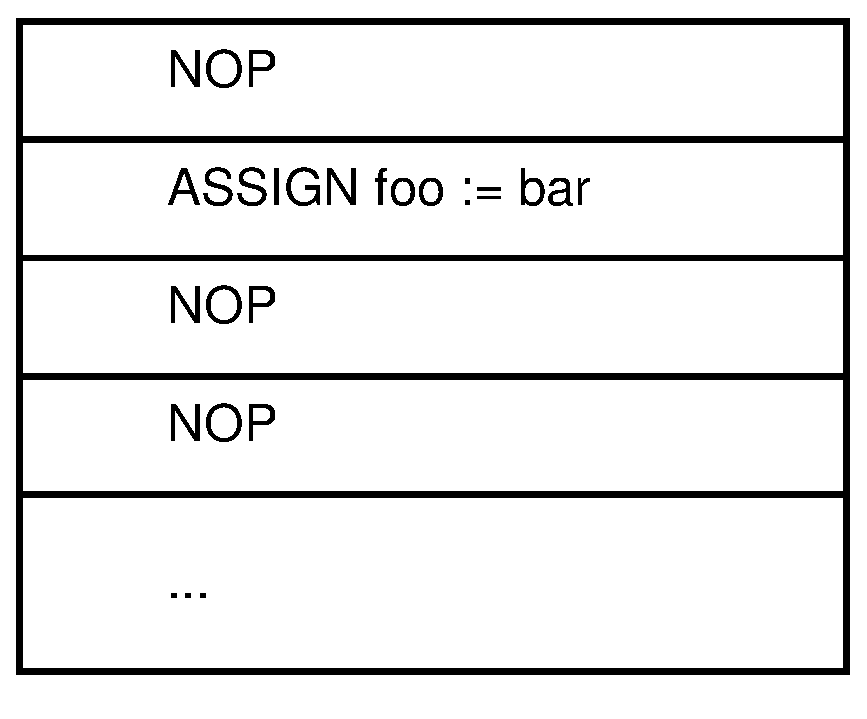
\includegraphics[scale=0.5]{figs/op-table.eps}
\caption{\label{fig:op-log}Operation Log}
\end{figure}

XXX: check retry semantic divide between paxos/db


\subsubsection{Reads}

For a distributed database there is the concept of \emph{fast reads} and \emph{slow reads}. A fast
read is a read that only examines the state of the database locally, without sending anything over
the network.  A slow read involves inserting an operation into the operation log in order to
ensure that the local copy of the database is up to date, then reading from that state.

A fast read has very low latency, as it does not need to send messages to any other nodes, but it
may return out of date data. A slow read forces us to actually examine the current state of the
database by inserting a \op{READ} operation, to ensure we have obtained all transactions issued
prior to our \op{READ}.

explain

In fact, I chose to use a \op{NOP} operation rather than a \op{READ} operation, although they
would semantically be the same (as other nodes do nothing on a \op{READ}), as I felt a \op{NOP}
better represented the operation being sent (do nothing).

explain about using nops to build knowledge of db

\subsubsection{Transactions}

My first implementation of transactions was a very na\"ive global lock. In order to start a
transaction, a node inserts the \op{TRYLOCK} operation. If, when the operation is inserted, the
number of \op{TRYLOCK}s is well-bracketed (ie, there is an equal number of lock takes and
releases), then the node was successful in taking the lock. While a node holds the lock, no other
node can perform an operation (the operations are inserted in the transaction log but ignored).

elaborate
diagram

\section{Paxos Implementation}

\subsection{State Machine Architecture}


Each of these acts like independant state machines.

Mixins
getattr

\begin{tabular}{ | c | c | p{7cm} | }
  \hline
  {\bf Message type} & {\bf Handler Class} & {\bf Message action} \\ \hline
  AcceptRequest & Acceptor & Respond with AcceptNotify (if valid) and accept Proposal. \\ \hline
  AcceptNotify & Learner & Record response and if a quorum has accepted that proposal, learn it. \\ \hline
  EHLO & Node & Respond with notify. \\ \hline
  Notify & Node & Add hosts to host list. \\ \hline
  Ping & Node & Send pong.  \\ \hline
  Pong & Node & Remove host from timeout list. \\ \hline
  Prepare & Acceptor & Respond with Promise (if valid). \\ \hline
  Promise & Proposer & Respond with AcceptRequest and deal with timeouts. \\ \hline
\end{tabular}



\section{Database Implementation}

SQL
How tools affected things
Optimisation - ``what it is''
Talk about iterations

SQL parser
- what it supports

-start up costs
  - ping time etc
  - inefficiencies
  - cf. ``supernodes'' vs DHTs to organise nodes

Talk about laptop breaking

\section{Testing}

I started off implementing unit tests for the 

\section{Commandline Tools}

bin/peval
etc etc
500 words


\cleardoublepage
\chapter{Evaluation}

This is where the second most amount of marks are gained.

Talk about scaling - different types of hierachy - DHT, supernodes etc

\section{Testing}

\begin{enumerate}
	\item unit test inertia
	\item test programs, see complex effects of single change.
	\item durable - network - stable storage
\end{enumerate}



\cleardoublepage
\chapter{Conclusion}

Conclude here.




\cleardoublepage

%%%%%%%%%%%%%%%%%%%%%%%%%%%%%%%%%%%%%%%%%%%%%%%%%%%%%%%%%%%%%%%%%%%%%
% the bibliography

\addcontentsline{toc}{chapter}{Bibliography}
\bibliography{refs}
\cleardoublepage

%%%%%%%%%%%%%%%%%%%%%%%%%%%%%%%%%%%%%%%%%%%%%%%%%%%%%%%%%%%%%%%%%%%%%
% the appendices
\appendix

\chapter{Project Proposal}

\vfil

\centerline{\Large Computer Science Project Proposal}
\vspace{0.4in}
\centerline{\Large PDB: A Distributed Database Based on Paxos}
\vspace{0.4in}
\centerline{\large Charlie Shepherd, Churchill College}
\vspace{0.3in}
\centerline{\large Originator: Charlie Shepherd}
\vspace{0.3in}
\centerline{\large 18$^{th}$ October 2012}

\vfil


\noindent
{\bf Project Supervisor:} Stephen Cross
\vspace{0.2in}

\noindent
{\bf Director of Studies:} Dr John Fawcett
\vspace{0.2in}
\noindent

\noindent
{\bf Project Overseers:} Dr~A.~Madhavapeddy \& Dr~M.~Kuhn


% Main document

\section*{Introduction, The Problem To Be Addressed}

{\em Paxos} is a protocol for achieving distributed consensus, developed by Leslie Lamport in 1991.

The motivation for Paxos as a protocol is that it is capable of handling failures that other
consensus protocols cannot. {\em Two Phase Commit} (2PC) and {\em Three Phase Commit} (3PC) are two common
protocols that can be used to ensure atomic commits in a distributed system.

2PC works by having a co-ordinator node contact every node and send a proposal message. Each node
must then either respond with a commit or abort message. However, 2PC suffers from several
problems, mainly that it is a blocking protocol. This means that if the co-ordinator fails, and
then a node subsequently fails, the network will deadlock, as 2PC is not able to recover from that
failure situation.

3PC is an extension to 2PC which endeavours to fix this limitation, at the expense of greater
latency, by adding a third roundtrip to confirm the commit to all nodes. This means that the
protocol is asynchronous, and that node failures cannot block the protocol or cause it to fail.
However, it still has its own limitations, in particular, in the event of a network partition. If
the network is partitioned so that in one partition all nodes vote ``commit'' and in the other all
nodes vote ``abort'' both partitions will initiate recovery, and when the network merges again the
system will be in an inconsistent state. This is the limitation that Paxos was intended to solve.

My project will be to design and implement a distributed database, built on the Paxos protocol.


\section*{Starting Point}

My starting point will be to study the Paxos protocol, as well as research distributed databases.
From there I will develop a library implementing Paxos, along with unit tests. I will then design
and implement a distributed database on the Paxos library. The challenge will be to implement a
complex distributed protocol and then utilise it for a database, as these are both areas I have
little experience of.

\section*{Resources Required}

I will mainly do my project on a virtual machine which is running on my own personal laptop.
The source code will be committed to a Git repository, which will be pushed to Bitbucket and my
own personal host. The virtual machine contents will be backed up on an external HDD for quick
recovery, although the git repository will be adequate for restoring my project if the system I am
developing it on fails.
I require no other special resources.

\section*{Work to be done}

The project breaks down into the following sub-projects:

\begin{enumerate}

\item A study of distributed algorithms and the Paxos protocol

\item A study of distributed databases

\item Implementing the Paxos protocol

\item Designing the distributed database

\item Implementing the distributed database

\item Evaluating the performance of the database

\end{enumerate}

\section*{Success Criteria for the Main Result}

In order for the project to be a success, the following must be true:

\begin{enumerate}

\item The project must correctly implement the Paxos protocol.
	The library must be capable of forming a running network,
	in particular dynamic leader election,
	as well as achieving consensus on a key/value store across the network.

\item The database must implement a subset of SQL, specifically:
\begin{enumerate}
\item A single table with a static name
\item SELECT/INSERT
\item WHERE
\item GROUP BY
\item ORDER BY
\item Aggregation
\end{enumerate}

\item The database must have all ACID properties, that is:
\begin{enumerate}
\item Atomic
\item Consistent
\item Isolated
\item Durable
\end{enumerate}

\end{enumerate}

\section*{Evaluation Topics}

There are several potential evaluation metrics for the project.

One major metric is transaction latency - the time for a transaction to be committed to the system. This
can be evaluated in a number of difference circumstances, including simulated node failure, leader
failure and network partition, and the results analysed to see how the system handles performance
under failure compared to normal conditions.

Another key metric is transaction throughput - the maximum number of transactions committed to the
network over a specified period of time. Again there are a number of different situations
throughput can be measured in, including load from one source, load from multiple sources and
load under failure.

I will also investigate the advantages of a distributed database over a normal single-server
database, particularly in terms of scalability. I will also consider how performance is affected
by the ratio of writing clients to reading clients.

\section*{Possible Extensions}

A clear possible extension is to investigate various different modifications to Paxos in order
to try to optimise the database for certain performance characteristics
(e.g. fast reads, but slow writes),
and to assess the usefulness and efficiency of these modifications.

Another possible extension is to investigate how the database performs when various ACID
properties are relaxed, and to measure and analyse how the performance gains compare with the
tradeoffs made.


\section*{Timetable: Workplan and Milestones to be achieved.}

\setlength\parindent{0pt}
\parskip = \baselineskip

Planned starting date is 19/10/2011.

\subsection*{Michaelmas Term}

{\bf 19/10/2012-01/11/2012} Research distributed algorithms and the Paxos protocol; design the
protocol implementation and library layout.

Milestone: A write up of the Paxos algorithm and a design document of the implementation.

{\bf 02/11/2012-15/11/2012} Begin the protocol implementation.

Milestone: Basic Paxos implementation.

{\bf 16/11/2012-29/11/2012} Finish implementation of Paxos library.

Milestone: Paxos implementation that can coordinate distributed leader election and achieve
consensus, including unit tests.

\subsection*{Christmas Vacation}

{\bf 30/11/2012-13/12/2012} Research distributed databases and design the database implementation.

Milestone: A write up of research on distributed databases and a design document for the database.

{\bf 14/12/2012-27/12/2012} Slack time/Revision/Holiday break.

{\bf 28/12/2012-10/01/2013} Prepare for progress report, start database implementation.

Milestone: Draft progress report, initial database implementation.

\subsection*{Lent Term}
{\bf 11/01/2013-24/01/2013} Write progress report, finish database implementation.

Milestone: Finished Progress report, fully functional database implementation.
Deadlines: Progress report deadline - 01/02/2013.

{\bf 25/01/2013-07/02/2013} Perform initial performance analysis on transaction, including
transaction latency and transaction throughput.

Milestone: Initial analysis data.

{\bf 08/02/2013-21/02/2013} Perform detailed performance analysis comparing distributed and
centralised servers, and on failing and partitioned networks.

Milestone: Analysis data on server models and on performance during failure.

{\bf 22/02/2013-07/03/2013} Investigate improvements to the protocol/implementation and their effect on
performance metrics.

Milestone: Improvements to protocol/implementation and revised performance data.

{\bf 08/03/2013-21/03/2013} Start dissertation.

Milestone: Draft Introduction and Preparation sections complete.

\subsection*{Easter Vacation}

{\bf 22/03/2013-04/04/2013} Finish writing up dissertation.

Milestone: Draft Implementation, Evaluation and Conclusion sections complete.

{\bf 05/04/2013-18/04/2013} Proof reading and then an early submission so as to concentrate on
examination revision.

Milestone: Finished dissertation.

\subsection*{Easter Term}
{\bf 19/04/2013-02/05/2013} Slack time/Revision/Holiday break.

{\bf 03/05/2013-16/05/2013} Slack time/Revision/Holiday break.

Deadlines: Official dissertation submission deadline - 17/05/2013.


\end{document}
